\documentclass[12pt,a4paper]{article}

\usepackage[utf8]{inputenc}
\usepackage[T1]{fontenc}
\usepackage{polski}
\usepackage{amsmath}
\usepackage{pgfplots}
\usepackage{tikz}
\usepackage{lmodern}	%fancy font
\usepackage{textcomp}
\usepackage{indentfirst}
\usepackage{graphicx}
\usepackage{caption}
\usepackage{subcaption}
\usepackage{here}
\usepackage{tabto}
\usepackage{multicol}

\setlength{\textheight}{24cm}
\setlength{\textwidth}{15.92cm}
\setlength{\footskip}{10mm}
\setlength{\oddsidemargin}{0mm}
\setlength{\evensidemargin}{0mm}
\setlength{\topmargin}{0mm}
\setlength{\headsep}{5mm}


\begin{document}
\title{Ogniwo słoneczne}
\date{11 października 2016}
\author{Miron Markowski, Łukasz Nawojowski}
\maketitle

\section{Cel ćwiczenia}

Zapoznanie się z działaniem ogniwa słonecznego i wyznaczenie:

\begin{itemize}
\item charakterystyk prądowo-napięciowych dla różnych rodzajów ogniw
przy ustalonym oświetleniu
\item Zależności gęstości prądu ogniwa jako funkcji napięcia na sekcję
\item Sprawności badanych ogniw
\end{itemize}



\section{Przebieg ćwiczenia}

\subsection{Układ doświadczalny}
Skonstruowano obwód z rys.1a i układ jak na rys. 1b.

\begin{figure}[H]
\centering
\begin{subfigure}{.5\textwidth}
  \centering
  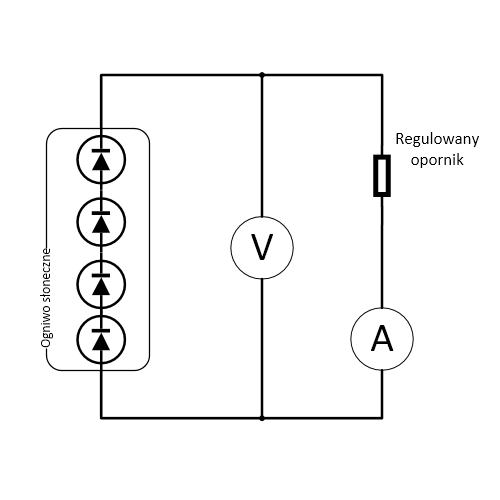
\includegraphics[width=1\textwidth]{img_fiz/Circuit}
  \caption{Obwód z ogniwem}
  \label{fig:sub1}
\end{subfigure}%
\begin{subfigure}{.5\textwidth}
  \centering
  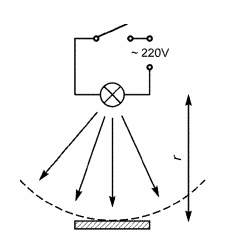
\includegraphics[width=1\textwidth]{img_fiz/Lamp}
  \caption{Lampa i ogniwo słoneczne}
  \label{fig:sub2}
\end{subfigure}
\caption{Układ doświadczalny}
\label{fig:test}
\end{figure}


\subsection{Wyniki pomiarów}

\begin{table}[H]
\centering
\caption{Natężenie światła}
\label{my-label}
\begin{tabular}{|p{3cm}|p{3cm}|}
\hline
$\phi$ {[}$W/m^2${]}	& $\phi$ śr. {[}$W/m^2${]}\\
\hline
60,0(4,0)				& 58,9(3,9)	\\
65,2(4,3)				&			\\
54,5(3,7)				&			\\
55,8(3,8)				&			\\
\hline   
\end{tabular}
\end{table}

\begin{table}[H]
\centering
\caption{Ogniwo polikrystaliczne - stałe}
\label{polistale}
\begin{tabular}{|p{2cm}|p{2cm}|p{2cm}|}
\hline
N & S {[}$cm^2${]} & N*S {[}$cm^2${]}   \\
\hline
8 & 7,8(1) & 62,4(1) \\
\hline
\end{tabular}
\end{table}

\begin{table}[H]
\centering
\caption{Ogniwo polikrystaliczne - pomiary}
\label{poliwyniki}
\begin{tabular}{|p{2cm}|p{2cm}|p{2cm}|p{2cm}|p{2cm}|}
\hline
I {[}$mA${]}	& U {[}$V${]}	& P  {[}$mW${]}	& U/N {[}$V${]}	& I/S {[}$A/m^2${]} \\
\hline
0,1243(20)		& 2,63(13)		& 0,33(2)		& 0,33(2)		& 0,159(4)\\
0,1694(30)		& 2,62(13)		& 0,44(2)		& 0,33(2)		& 0,217(4)\\
0,20(10)		& 2,61(13)		& 0,52(27)		& 0,33(2)		& 0,26(13)\\
0,60(11)		& 2,53(13)		& 1,52(28)		& 0,32(2)		& 0,77(14)\\
1,00(11)		& 2,46(12)		& 2,46(30)		& 0,31(2)		& 1,28(14)\\
1,43(11)		& 2,37(12)		& 3,39(32)		& 0,30(2)		& 1,83(15)\\
1,63(12)		& 2,33(12)		& 3,80(34)		& 0,29(2)		& 2,09(15)\\
1,85(12)		& 2,28(12)		& 4,22(35)		& 0,29(2)		& 2,37(15)\\
2,00(12)		& 2,25(12)		& 4,50(36)		& 0,28(2)		& 2,56(16)\\
2,24(12)		& 2,18(12)		& 4,88(38)		& 0,27(2)		& 2,87(16)\\
2,43(12)		& 2,12(12)		& 5,15(40)		& 0,27(2)		& 3,12(16)\\
2,69(13)		& 2,05(12)		& 5,51(42)		& 0,26(2)		& 3,45(17)\\
2,99(13)		& 1,966(30)		& 5,88(27)		& 0,246(4)		& 3,83(17)\\
3,22(13)		& 1,892(29)		& 6,09(27)		& 0,237(4)		& 4,13(18)\\
3,37(13)		& 1,89(12)		& 6,37(47)		& 0,24(1)		& 4,32(18)\\
3,55(14)		& 1,735(27)		& 6,16(25)		& 0,217(3)		& 4,55(18)\\
3,59(14)		& 1,80(12)		& 6,46(49)		& 0,23(1)		& 4,60(18)\\
3,87(14)		& 1,515(25)		& 5,86(23)		& 0,189(3)		& 4,96(19)\\
4,07(14)		& 1,329(23)		& 5,41(21)		& 0,166(3)		& 5,22(19)\\
4,25(14)		& 1,109(21)		& 4,71(18)		& 0,139(3)		& 5,45(20)\\
4,41(14)		& 0,793(18)		& 3,50(14)		& 0,099(2)		& 5,65(20)\\
4,51(15)		& 0,671(17)		& 3,03(12)		& 0,084(2)		& 5,78(20)\\
4,69(15)		& 0,530(15)		& 2,49(11)		& 0,066(2)		& 6,01(20)\\
\hline
\end{tabular}
\end{table}

\newpage

\begin{table}[H]
\centering
\caption{Ogniwo monokrystaliczne - stałe}
\label{monostale}
\begin{tabular}{|p{2cm}|p{2cm}|p{2cm}|}
\hline
N & S {[}$cm^2${]} & N*S {[}$cm^2${]}   \\
\hline
1 & 63,0(1) & 63,0(1) \\
\hline
\end{tabular}
\end{table}

\begin{table}[H]
\centering
\caption{Ogniwo monokrystaliczne - pomiary}
\label{mono}
\begin{tabular}{|p{2cm}|p{2cm}|p{2cm}|p{2cm}|p{2cm}|}
\hline
I {[}$mA${]}	& U {[}$V${]}	& P  {[}$mW${]}	& U/N {[}$V${]} & I/S {[}$A/m^2${]} \\ 
\hline
0,6(1,0)		& 0,46(1)		& 0,27(46)		& 0,46(1)		& 0,10(16)\\
1,0(1,0)		& 0,46(1)		& 0,46(46)		& 0,46(1)		& 0,16(16)\\
1,7(1,0)		& 0,46(1)		& 0,78(47)		& 0,46(1)		& 0,27(16)\\
2,2(1,0)		& 0,46(1)		& 1,01(47)		& 0,46(1)		& 0,35(16)\\
3,6(1,0)		& 0,46(1)		& 1,64(48)		& 0,46(1)		& 0,57(16)\\
5,2(1,1)		& 0,45(1)		& 2,36(48)		& 0,45(1)		& 0,83(17)\\
7,1(1,1)		& 0,45(1)		& 3,21(49)		& 0,45(1)		& 1,13(17)\\
10,6(1,1)		& 0,45(1)		& 4,76(52)		& 0,45(1)		& 1,68(18)\\
15,7(1,1)		& 0,44(1)		& 6,96(56)		& 0,44(1)		& 2,49(18)\\
\hline
\end{tabular}
\end{table}


\begin{center}
\begin{tikzpicture}[scale=1.5]
\begin{axis}[
    title={Zależność gęstości prądu od napięcia na sekcję},
    xlabel={Napięcie na sekcję U/N [V]},
    ylabel={Gęstość prądu j [$A/m^2$]},
    xmin=0, xmax=0.5,
    ymin=0, ymax=8,
    xtick={0,0.1,0.2,0.3,0.4, 0.5},
    ytick={0,1,2,3,4,5,6,7, 8, 9},
    legend image post style=only marks,
    legend pos=north east,
    grid=major,
    grid style=dashed,
]
 
\addplot+[
    color=blue,
    mark=x,
    draw=none,
    error bars/.cd,
    x dir=both,x explicit,
    y dir=both,y explicit,
    ]
    coordinates {
    (0.33,	0.159) +- (0.02,0.004)
	(0.33,	0.217) +- (0.02,0.004)
	(0.33,	0.26) +- (0.02,0.13)
	(0.32,	0.77) +- (0.02,0.14)
	(0.31,	1.28) +- (0.02,0.14)
	(0.30,	1.83) +- (0.02,0.15)
	(0.29,	2.09) +- (0.02,0.15)
	(0.29,	2.37) +- (0.02,0.15)
	(0.28,	2.56) +- (0.02,0.16)
	(0.27,	2.87) +- (0.02,0.16)
	(0.27,	3.12) +- (0.02,0.16)
	(0.26,	3.45) +- (0.02,0.17)
	(0.246,	3.83) +- (0.004,0.17)
	(0.237,	4.13) +- (0.004,0.18)
	(0.24,	4.32) +- (0.01,0.18)
	(0.23,	4.60) +- (0.01,0.18)
	(0.217,	4.55) +- (0.003,0.18)
	(0.189,	4.96) +- (0.003,0.19)
	(0.166,	5.22) +- (0.003,0.19)
	(0.139,	5.45) +- (0.003,0.20)
	(0.099,	5.65) +- (0.002,0.20)
	(0.084,	5.78) +- (0.002,0.20)
	(0.066,	6.01) +- (0.002,0.20)
    };
    \addlegendentry{Polikrystaliczne}
    
    \addplot+[
    color=red,
    mark=x,
    draw=none,
    error bars/.cd,
    x dir=both,x explicit,
    y dir=both,y explicit,
    ]
    coordinates {
    (0.46, 0.10) +- (0.01,0.16)
	(0.46, 0.16) +- (0.01,0.16)
	(0.46, 0.27) +- (0.01,0.16)
	(0.46, 0.35) +- (0.01,0.16)
	(0.46, 0.57) +- (0.01,0.16)
	(0.45, 0.83) +- (0.01,0.17)
	(0.45, 1.13) +- (0.01,0.17)
	(0.45, 1.68) +- (0.01,0.18)
	(0.44, 2.49) +- (0.01,0.18)
    };
    \addlegendentry{Monokrystaliczne}
 
\end{axis}
\end{tikzpicture}
\end{center}

\newpage

\subsection{Omówienie wyników}
Pomiar napięcia i natężenia dla ogniwa polikrystalicznego dał o wiele ciekawszą krzywą, mówiącą więcej o ogólnym kształcie funkcji niż dla ogniwa monokrystalicznego, gdyż zakres oporu jakim dysponowaliśmy nie pozwolił na znaczne zmiany napięcia na tym ogniwie (różnica 0,02 V między napięciami na najmniejszym a największym możliwym oporze). Dlatego też choć maksymalna moc dla obu ogniw jest podobna, około 7 mW, można podejrzewać, że maksimum mocy dla ogniwa monokrystalicznego można zaobserwować dla oporu mniejszego niż najmniejszy dostępny przy oporniku, którym dysponowaliśmy. \\
W punkcie największej zmierzonej mocy ogniwo monokrystaliczne ma większe napięcie na sekcję, zaś ogniwo polikrystaliczne ma większą gęstość prądu.\\\\
Sprawność ogniwa wynosi:
$\eta = \dfrac{P}{P_{\text{źródła}}} = \dfrac{P}{\phi \times S}$ \\
zatem dla ogniwa:\\
\begin{itemize}
\item polikrystalicznego:
$\eta = \dfrac{6,46 \times 10^{-3} W}{58,9 \frac{W}{m^2} \times 62,4 \times 10^{-4} m^2} \approx 1,76(18) \%$ \\\\
\item monokrystalicznego:
$\eta = \dfrac{6,96 \times 10^{-3} W}{58,9 \frac{W}{m^2} \times 62,4 \times 10^{-4} m^2} \approx 1,88(20) \% $
\end{itemize}
Tak niska sprawność może wynikać np. z faktu, że ogniwo jest już stare i zużyte, może mieć też zanieczyszczoną powierzchnię, ponadto światło lampy mogło mieć niewłaściwą długość fali, przez co efekt fotowoltaiczny nie był odpowiednio wydajny.

\subsection{Dyskusja niepewności i błędów}
Na używanych elektronicznych przyrządach pomiarowych nie naniesiono informacji o ich dokładności, dlatego niepewności oszacowano na podstawie obserwacji działania przyrządów w trakcie wykonywania pomiarów (np. porównanie zbliżonych wartości pomiaru na różnych zakresach) i typowych charakterystyk przyrządów pomiarowych danego typu.\\
Niepewności pomiaru napięcia oraz natężenia prądu, a także natężenia światła obliczono zgodnie z wzorem:
$$u(x) = \frac{\Delta x}{\sqrt{3}},\ \Delta x = C_1 \times x + C_2 \times r^x
\text{, gdzie: $C_1, C_2$ - stałe przyrządu, $r^x$ - zakres miernika}$$

Zakresy mierników podane są w arkuszu z wynikami pomiarów, natomiast stałe $C_1$ oraz $C_2$ dobrano jak następuje:
\begin{itemize}
\TabPositions{3cm}
\item amperomierz:\tab$C_1^I = 1\%$, $C_2^I = 0,5\%$
\item woltomierz:\tab$C_1^U = 1\%$, $C_2^U = 0,5\%$
\item luksomierz:\tab$C_1^\phi = 5\%$, $C_2^\phi = 0,5\%$
\end{itemize}

Ostateczna wartość natężenia światła $\phi$ jest średnią z czterech pomiarów, jednak każdy z nich został wykonany przy innym boku ogniwa, dlatego nie potraktowano ich jako serii statystycznej jednej wielkości, lecz zastosowano oszacowanie niepewności typu B do uzyskanej wartości średniej, tak jakby to ona była wynikiem pomiaru.

Całkowita powierzchnia ogniwa $S$ była dana na płytce z ogniwem bez informacji o dokładności, zatem za jej niepewność przyjęto ostatnią podaną cyfrę.

Niepewności obliczono według następujących wzorów:\\
$$u(I) = \frac{1}{\sqrt{3}} (C_1^I \times I + C_2^I \times r^I)$$
$$u(U) = \frac{1}{\sqrt{3}} (C_1^U \times U + C_2^U \times r^U)$$
$$u(\phi) = \frac{1}{\sqrt{3}} (C_1^\phi \times \phi + C_2^\phi \times r^\phi)$$
$$u_c(P) = u_c(U \times I) = \sqrt{(I \times u(U))^2 + (U \times u(I))^2}$$
$$u(U/N) = u(U)/N$$
$$u_c(I/S) = \sqrt{((1/S) \times u(I))^2 + ((I/S^2) \times u(S))^2}$$
$u_c(\eta) = u_c(P/(\phi \times S))\\ \text{\qquad\ } = \sqrt{((1/(\phi \times S) \times u_c(P))^2 + (P/(\phi^2 \times S) \times u(\phi))^2 + (P/(\phi \times S^2) \times u(S))^2}$\\

Należy odnotować, że opornik na płytce z ogniwem monokrystalicznym był rozstrojony, tzn. przy kręceniu jego gałką regulującą, rezystancja rosła zgodnie z oczekiwaniami, w pewnym momencie gwałtownie malała, a potem znów gwałtownie rosła, by powrócić do poziomu sprzed spadku. Z tego powodu część wyników pomiaru odrzucono jako nieweryfikowalne bez użycia innego opornika. Również dlatego zakres amperomierza użyty przy pomiarach na ogniwie monokrystalicznym jest nieadekwatny w stosunku do nieodrzuconej części zmierzonych natężeń, przez co ich niepewności są stosunkowo duże.

\end{document}
